%% AdaPres manuscript -- Springer Nature sn-jnl template (v3.1).
%% Every result is a macro from numbers.tex / numbers_v2.tex, generated from results/ by
%% paper/make_numbers.py and paper/make_v2.py. Tables in tables/ and figures in figs/ are generated
%% too (scripts/build_springer.py copies them here). Do not type results by hand.
\documentclass[pdflatex,sn-mathphys-num]{sn-jnl}
\usepackage{graphicx}
\usepackage{amsmath,amssymb,amsfonts}
\usepackage{booktabs}
\usepackage{xcolor}
\usepackage{textcomp}
\usepackage{newunicodechar}
\newunicodechar{−}{\ensuremath{-}}
\newunicodechar{Δ}{\ensuremath{\Delta}}
\newunicodechar{≥}{\ensuremath{\geq}}
\newunicodechar{·}{\ensuremath{\cdot}}
\newunicodechar{×}{\ensuremath{\times}}
\newunicodechar{…}{\ldots}
\newunicodechar{§}{\S}
\raggedbottom

% generated by paper/make_numbers.py from results/ -- do not edit
% results commit 4e35b3e1d68453b5e17eb15c09293e3d94eaabe3
\newcommand{\BootResamples}{1{,}000}
\newcommand{\CalibClips}{20}
\newcommand{\CalibConfigs}{32{,}376}
\newcommand{\CalibDropMain}{0.44}
\newcommand{\CommitRun}{4e35b3e1}
\newcommand{\CueCostMs}{2.70}
\newcommand{\DeltaPts}{0.5}
\newcommand{\DiffAdaptiveFPsixteenCIHi}{-0.13}
\newcommand{\DiffAdaptiveFPsixteenCILo}{-2.42}
\newcommand{\DiffAdaptiveFPsixteenMean}{-1.00}
\newcommand{\DiffAdaptiveINTeightCIHi}{+0.27}
\newcommand{\DiffAdaptiveINTeightCILo}{-0.53}
\newcommand{\DiffAdaptiveINTeightMean}{+0.03}
\newcommand{\DiffAdaptiveRandomIidCIHi}{+0.21}
\newcommand{\DiffAdaptiveRandomIidCILo}{-1.38}
\newcommand{\DiffAdaptiveRandomIidMean}{-0.38}
\newcommand{\DiffAdaptiveRandomMatchedCIHi}{+0.27}
\newcommand{\DiffAdaptiveRandomMatchedCILo}{-0.70}
\newcommand{\DiffAdaptiveRandomMatchedMean}{+0.01}
\newcommand{\DiffOracleFPsixteenCIHi}{+0.48}
\newcommand{\DiffOracleFPsixteenCILo}{-0.55}
\newcommand{\DiffOracleFPsixteenMean}{-0.10}
\newcommand{\DriftFPsixteen}{0.08}
\newcommand{\DriftINTeight}{0.21}
\newcommand{\DropAdaptiveVsFPsixteen}{0.90}
\newcommand{\DropINTeightVsFPsixteen}{0.94}
\newcommand{\EDynAdaptPipe}{178}
\newcommand{\EDynAdaptSeq}{79}
\newcommand{\EDynFPsixteen}{204}
\newcommand{\EDynFPthirtytwo}{365}
\newcommand{\EDynINTeight}{167}
\newcommand{\ETotalAdaptPipe}{363}
\newcommand{\ETotalAdaptSeq}{369}
\newcommand{\ETotalFPsixteen}{393}
\newcommand{\ETotalFPthirtytwo}{723}
\newcommand{\ETotalINTeight}{333}
\newcommand{\EngineMsFPsixteen}{2.70}
\newcommand{\EngineMsFPthirtytwo}{7.78}
\newcommand{\EngineMsINTeight}{1.99}
\newcommand{\EngineSavingINTeightMs}{0.71}
\newcommand{\EngineSpeedupINTeightPct}{26}
\newcommand{\FpsAdaptPipe}{175}
\newcommand{\FpsAdaptSeq}{112}
\newcommand{\FpsFPsixteen}{172}
\newcommand{\FpsFPthirtytwo}{91}
\newcommand{\FpsINTeight}{197}
\newcommand{\FracINTeightAdaptive}{0.96}
\newcommand{\FracINTeightFixedFPsixteen}{0.00}
\newcommand{\FracINTeightFixedFPthirtytwo}{0.00}
\newcommand{\FracINTeightFixedINTeight}{1.00}
\newcommand{\FracINTeightOracle}{0.63}
\newcommand{\FracINTeightRandomIid}{0.50}
\newcommand{\FracINTeightRandomMatched}{0.96}
\newcommand{\HFourEasyShare}{0.505}
\newcommand{\HFourResult}{supported}
\newcommand{\HOneResult}{not supported}
\newcommand{\HThreeResult}{supported}
\newcommand{\HTwoResult}{not supported}
\newcommand{\INTeightETotalRedPct}{15}
\newcommand{\INTeightLatRedPct}{13}
\newcommand{\LatAdaptPipe}{5.54}
\newcommand{\LatAdaptSeq}{8.85}
\newcommand{\LatFPsixteen}{5.78}
\newcommand{\LatFPthirtytwo}{11.02}
\newcommand{\LatINTeight}{5.03}
\newcommand{\LatPninetyfiveAdaptPipe}{6.57}
\newcommand{\LatPninetyfiveAdaptSeq}{9.50}
\newcommand{\LatPninetyfiveFPsixteen}{6.07}
\newcommand{\LatPninetyfiveFPthirtytwo}{11.44}
\newcommand{\LatPninetyfiveINTeight}{5.34}
\newcommand{\LiveAgreementPct}{100}
\newcommand{\LiveFrames}{1{,}924}
\newcommand{\MapAdaptive}{25.81}
\newcommand{\MapAdaptiveCIHi}{36.06}
\newcommand{\MapAdaptiveCILo}{22.18}
\newcommand{\MapAdaptiveCrowded}{23.82}
\newcommand{\MapAdaptiveEasy}{33.91}
\newcommand{\MapAdaptiveNight}{11.64}
\newcommand{\MapAdaptiveSceneChange}{20.65}
\newcommand{\MapChangeKEight}{+0.14}
\newcommand{\MapChangeKFive}{+0.02}
\newcommand{\MapChangeKThree}{-0.00}
\newcommand{\MapChangeKTwo}{+0.00}
\newcommand{\MapFiftyAdaptive}{41.23}
\newcommand{\MapFiftyFixedFPsixteen}{42.95}
\newcommand{\MapFiftyFixedFPthirtytwo}{42.95}
\newcommand{\MapFiftyFixedINTeight}{41.27}
\newcommand{\MapFiftyOracle}{43.28}
\newcommand{\MapFiftyRandomIid}{42.04}
\newcommand{\MapFiftyRandomMatched}{41.26}
\newcommand{\MapFixedFPsixteen}{26.71}
\newcommand{\MapFixedFPsixteenCIHi}{36.93}
\newcommand{\MapFixedFPsixteenCILo}{22.99}
\newcommand{\MapFixedFPsixteenCrowded}{24.50}
\newcommand{\MapFixedFPsixteenEasy}{34.01}
\newcommand{\MapFixedFPsixteenNight}{12.55}
\newcommand{\MapFixedFPsixteenSceneChange}{21.61}
\newcommand{\MapFixedFPthirtytwo}{26.70}
\newcommand{\MapFixedFPthirtytwoCIHi}{36.93}
\newcommand{\MapFixedFPthirtytwoCILo}{22.99}
\newcommand{\MapFixedFPthirtytwoCrowded}{24.50}
\newcommand{\MapFixedFPthirtytwoEasy}{33.98}
\newcommand{\MapFixedFPthirtytwoNight}{12.59}
\newcommand{\MapFixedFPthirtytwoSceneChange}{21.80}
\newcommand{\MapFixedINTeight}{25.76}
\newcommand{\MapFixedINTeightCIHi}{36.10}
\newcommand{\MapFixedINTeightCILo}{22.08}
\newcommand{\MapFixedINTeightCrowded}{23.53}
\newcommand{\MapFixedINTeightEasy}{33.91}
\newcommand{\MapFixedINTeightNight}{11.61}
\newcommand{\MapFixedINTeightSceneChange}{18.68}
\newcommand{\MapOracle}{26.67}
\newcommand{\MapOracleCIHi}{37.09}
\newcommand{\MapOracleCILo}{22.92}
\newcommand{\MapOracleCrowded}{24.34}
\newcommand{\MapOracleEasy}{34.24}
\newcommand{\MapOracleNight}{12.31}
\newcommand{\MapOracleSceneChange}{21.56}
\newcommand{\MapRandomIid}{26.16}
\newcommand{\MapRandomIidCIHi}{36.40}
\newcommand{\MapRandomIidCILo}{22.46}
\newcommand{\MapRandomIidCrowded}{23.95}
\newcommand{\MapRandomIidEasy}{33.84}
\newcommand{\MapRandomIidNight}{12.05}
\newcommand{\MapRandomIidSD}{0.11}
\newcommand{\MapRandomIidSceneChange}{20.33}
\newcommand{\MapRandomMatched}{25.77}
\newcommand{\MapRandomMatchedCIHi}{36.12}
\newcommand{\MapRandomMatchedCILo}{22.08}
\newcommand{\MapRandomMatchedCrowded}{23.55}
\newcommand{\MapRandomMatchedEasy}{33.85}
\newcommand{\MapRandomMatchedNight}{11.63}
\newcommand{\MapRandomMatchedSD}{0.06}
\newcommand{\MapRandomMatchedSceneChange}{18.91}
\newcommand{\SceneChangeFrames}{160}
\newcommand{\SwitchPenaltyMs}{-0.08}
\newcommand{\SwitchRateAdaptive}{1.48}
\newcommand{\SwitchRateFixedFPsixteen}{0.00}
\newcommand{\SwitchRateFixedFPthirtytwo}{0.00}
\newcommand{\SwitchRateFixedINTeight}{0.00}
\newcommand{\SwitchRateKEight}{1.03}
\newcommand{\SwitchRateKFive}{1.18}
\newcommand{\SwitchRateKOne}{1.48}
\newcommand{\SwitchRateKThree}{1.21}
\newcommand{\SwitchRateKTwo}{1.30}
\newcommand{\SwitchRateOracle}{34.08}
\newcommand{\SwitchRateRandomIid}{50.13}
\newcommand{\SwitchRateRandomMatched}{1.45}
\newcommand{\TestClips}{40}
\newcommand{\TestFrames}{7{,}796}

% generated by paper/make_v2.py from results/ -- do not edit
% results commit 2f0c780d62ea19e97b33596350f60a63e74a218b
\newcommand{\CapturedFiftyPct}{-4}
\newcommand{\CapturedSeventyFivePct}{-5}
\newcommand{\CapturedTwentyFivePct}{-7}
\newcommand{\CommitVTwoRun}{2f0c780d}
\newcommand{\DiffPOneCIHi}{+0.38}
\newcommand{\DiffPOneCILo}{-0.49}
\newcommand{\DiffPOneMean}{-0.03}
\newcommand{\DiffPThreeCIHi}{+0.56}
\newcommand{\DiffPThreeCILo}{-0.14}
\newcommand{\DiffPThreeMean}{+0.18}
\newcommand{\DiffPTwoHighCIHi}{+0.42}
\newcommand{\DiffPTwoHighCILo}{-1.08}
\newcommand{\DiffPTwoHighMean}{-0.11}
\newcommand{\DiffPTwoLowCIHi}{+0.22}
\newcommand{\DiffPTwoLowCILo}{-0.15}
\newcommand{\DiffPTwoLowMean}{+0.02}
\newcommand{\DiffVTwoFPsixteenCIHi}{+0.04}
\newcommand{\DiffVTwoFPsixteenCILo}{-1.07}
\newcommand{\DiffVTwoFPsixteenMean}{-0.44}
\newcommand{\DiffVTwoINTeightCIHi}{+0.90}
\newcommand{\DiffVTwoINTeightCILo}{-0.13}
\newcommand{\DiffVTwoINTeightMean}{+0.40}
\newcommand{\FracLaggedFifty}{0.66}
\newcommand{\FracLaggedSeventyFive}{0.74}
\newcommand{\FracLaggedTwentyFive}{0.22}
\newcommand{\FracOracleFifty}{0.50}
\newcommand{\FracOracleSeventyFive}{0.75}
\newcommand{\FracOracleTwentyFive}{0.25}
\newcommand{\FracRandomFifty}{0.42}
\newcommand{\FracRandomSeventyFive}{0.60}
\newcommand{\FracRandomTwentyFive}{0.17}
\newcommand{\FracVOneFifty}{0.66}
\newcommand{\FracVOneSeventyFive}{0.86}
\newcommand{\FracVOneTwentyFive}{0.36}
\newcommand{\FracVTwoFifty}{0.41}
\newcommand{\FracVTwoSeventyFive}{0.60}
\newcommand{\FracVTwoTwentyFive}{0.18}
\newcommand{\MapLaggedFifty}{26.43}
\newcommand{\MapLaggedSeventyFive}{26.27}
\newcommand{\MapLaggedTwentyFive}{26.61}
\newcommand{\MapOracleFifty}{26.99}
\newcommand{\MapOracleSeventyFive}{26.59}
\newcommand{\MapOracleTwentyFive}{26.86}
\newcommand{\MapRandomFifty}{26.32}
\newcommand{\MapRandomSDFifty}{0.09}
\newcommand{\MapRandomSDSeventyFive}{0.19}
\newcommand{\MapRandomSDTwentyFive}{0.10}
\newcommand{\MapRandomSeventyFive}{26.13}
\newcommand{\MapRandomTwentyFive}{26.58}
\newcommand{\MapVFixedFPsixteen}{26.69}
\newcommand{\MapVFixedFPthirtytwo}{26.70}
\newcommand{\MapVFixedINTeight}{25.90}
\newcommand{\MapVOneFifty}{26.17}
\newcommand{\MapVOneSeventyFive}{26.14}
\newcommand{\MapVOneTwentyFive}{26.42}
\newcommand{\MapVTwoFifty}{26.30}
\newcommand{\MapVTwoSeventyFive}{26.10}
\newcommand{\MapVTwoTwentyFive}{26.56}
\newcommand{\SwitchVTwoFifty}{21.4}
\newcommand{\SwitchVTwoSeventyFive}{3.3}
\newcommand{\SwitchVTwoTwentyFive}{2.2}
\newcommand{\VControllerMsPipe}{2.29}
\newcommand{\VCueWaitMsPipe}{0.05}
\newcommand{\VCueWaitMsSeq}{2.73}
\newcommand{\VDriftINTeight}{0.41}
\newcommand{\VDropINTeightPts}{0.79}
\newcommand{\VEDynAlternation}{192}
\newcommand{\VEDynFPsixteen}{219}
\newcommand{\VEDynINTeight}{157}
\newcommand{\VEDynVTwoPipe}{127}
\newcommand{\VEDynVTwoSeq}{72}
\newcommand{\VETotalAlternation}{351}
\newcommand{\VETotalFPsixteen}{388}
\newcommand{\VETotalINTeight}{305}
\newcommand{\VETotalVTwoPipe}{395}
\newcommand{\VETotalVTwoSeq}{439}
\newcommand{\VEnergyClips}{6}
\newcommand{\VHeadroomFiftyPts}{0.67}
\newcommand{\VINTeightETotalRedPct}{21}
\newcommand{\VINTeightLatRedPct}{12}
\newcommand{\VLatAlternation}{5.45}
\newcommand{\VLatFPsixteen}{5.63}
\newcommand{\VLatINTeight}{4.93}
\newcommand{\VLatVTwoPipe}{8.94}
\newcommand{\VLatVTwoSeq}{11.91}
\newcommand{\VLiveAgreementPct}{100}
\newcommand{\VMeasFracINTeight}{0.37}
\newcommand{\VMeasSwitchRate}{24.3}
\newcommand{\VPFiveResult}{not supported}
\newcommand{\VPOneResult}{not supported}
\newcommand{\VSpearman}{0.06}


\begin{document}

\title[Content-aware INT8/FP16 switching: a pre-registered negative result]{Does Content-Aware Precision Switching Pay Off for Real-Time Object Detection? A Pre-Registered Negative Result on Driving Video}

%% Corresponding author not yet designated (author.md: ask, do not invent). Mark with \author* once confirmed.
\author[1]{\fnm{Vinay} \sur{Kamble}}\email{vinaykamble289@gmail.com}
\author[1]{\fnm{Aisshwarya} \sur{Gurav}}\email{aisshwaryagurav@gmail.com}
\author[1]{\fnm{Shrejal} \sur{Bhosale}}\email{bhosaleshrejal@gmail.com}

\affil[1]{\orgdiv{Department of Computer Science and Engineering (Artificial Intelligence and Machine Learning)}, \orgname{KIT's College of Engineering}, \orgaddress{\city{Kolhapur}, \state{Maharashtra}, \country{India}}}

\abstract{Running a detector at reduced numerical precision on frames that tolerate it, and at full precision elsewhere, promises most of the speed and energy of INT8 inference with the accuracy of FP16, provided a controller can tell the frames apart. We test this premise for YOLO11s on BDD100K MOT driving video on one NVIDIA T4 with TensorRT, under a protocol that fixed hypotheses, calibration on held-out clips and a one-shot test evaluation in advance. A content-cue controller (motion, clutter, detection count, confidence, scene change), calibrated and locked on calibration clips, lost \DropAdaptiveVsFPsixteen{} points of mAP@0.5:0.95 against FP16 and could not be distinguished from fixed INT8 or from switching at random with the same INT8 share. A pre-registered follow-up with a learned per-frame risk estimator under fixed INT8 budgets also failed to beat matched random placement (difference $\DiffPOneMean$ points, 95\% CI $[\DiffPOneCILo, \DiffPOneCIHi]$), although a ground-truth oracle shows \VHeadroomFiftyPts{} points of headroom at a 50\% budget. Switching between engines is cheap, but deciding is not: the controller's CPU work made adaptive inference slower than FP16 (\VLatVTwoPipe{} vs \VLatFPsixteen{} ms per frame). On this setup, fixed INT8 is the better choice: \VDropINTeightPts{} points lower mAP, with \VINTeightLatRedPct\% lower latency and \VINTeightETotalRedPct\% lower GPU board energy per frame than FP16.}

\keywords{Mixed-precision inference, INT8 quantization, adaptive inference, video object detection, energy measurement, negative result, pre-registration}

\maketitle

%% =====================================================================================
\section{Introduction}\label{sec:intro}

Post-training INT8 quantization makes convolutional detectors faster and cheaper to run on GPUs with integer tensor cores~\cite{jacob2018quantization,nagel2021whitepaper}, at the price of a small, but not uniform, loss of accuracy. If that loss were concentrated in identifiable frames, such as crowded scenes, night driving or scene cuts, a controller could run INT8 on the remaining frames and FP16 on the difficult ones, keeping FP16 accuracy at close to INT8 cost. This idea is close to adaptive configuration in video analytics~\cite{jiang2018chameleon,chin2019adascale,xu2020approxdet} and to input-dependent precision~\cite{liu2022dqnet,sun2021videoiq}, but it operates on the cheapest possible knob: two pre-built engines of the same network, switched per frame.

We asked whether this works in a realistic setting and evaluated it in a way that makes a negative answer credible. Hypotheses, the accuracy tolerance $\delta = \DeltaPts$ points, the calibration procedure and the statistical tests were fixed before any test data were seen. Every threshold and weight was fit on calibration clips, and the test clips were scored once per locked configuration. When a review pointed out that the first controller collapsed to near-constant INT8, we pre-registered a second controller and its tests in an addendum before running it.

The answer is negative on this setup, and we report it as such. Our contributions are:
\begin{itemize}
\item A pre-registered, replay-plus-live evaluation protocol for per-frame precision switching. It includes a cost-matched random baseline, a ground-truth oracle as an upper bound, cluster-bootstrap confidence intervals over clips, and live measurements of latency and GPU board energy.
\item Evidence that neither a hand-weighted content-cue controller nor a learned per-frame risk estimator places INT8 frames better than chance on BDD100K MOT driving video, even though an oracle shows that headroom exists.
\item A cost decomposition showing that switching between resident engines is nearly free, while the controller's own CPU work exceeds the INT8 saving, which makes adaptive inference slower than fixed FP16.
\item Code, locked configurations with hashes, and every result file needed to reproduce the tables and figures.
\end{itemize}

%% =====================================================================================
\section{Related work}\label{sec:related}

\paragraph{Quantization.} Integer-only inference~\cite{jacob2018quantization} and post-training quantization~\cite{nagel2021whitepaper} make INT8 detectors practical, and TensorRT builds INT8 and FP16 engines from a trained network~\cite{nvidia_tensorrt_docs}. Mixed-precision methods such as HAQ~\cite{wang2019haq} choose bit-widths per layer offline, whereas we switch the precision of the whole network per frame at run time.

\paragraph{Input-adaptive precision.} AdaBits~\cite{jin2020adabits} trains one network whose bit-width can be switched at deployment but does not decide when to switch. DQNet~\cite{liu2022dqnet} trains a bit-controller with the network to pick per-layer bit-widths for each image, and VideoIQ~\cite{sun2021videoiq} trains a policy that selects the precision of each video frame for action recognition. These methods learn the policy together with the model and report gains. We study the post-hoc setting that deployment toolchains offer: two fixed post-training engines and a controller that is added afterwards. There, our results show no gain over random placement.

\paragraph{Adaptive video analytics and detection.} Chameleon~\cite{jiang2018chameleon} re-profiles resolution, frame rate and model per video segment and stresses that profiling itself is costly. AdaScale~\cite{chin2019adascale} picks the input scale per frame with a learned regressor and improves both speed and accuracy. ApproxDet~\cite{xu2020approxdet} selects approximate detection configurations from content and resource contention, and LiteReconfig~\cite{xu2022litereconfig} adds a cost--benefit analysis of which content features are worth computing, accounting for switching overhead. Remix~\cite{jiang2021remix} allocates detectors of different sizes to regions of high-resolution frames under a latency budget, and DynamicDet~\cite{lin2023dynamicdet} routes easy images through a cheaper path of a cascaded YOLO detector. Our controller is closest to ApproxDet, and our cost finding matches the motivation of LiteReconfig: on a T4 the features needed to decide cost more than INT8 saves.

%% =====================================================================================
\section{Method}\label{sec:method}

\subsection{Precision levels and replay}
The detector is run as TensorRT engines at FP32, FP16 and INT8; INT8 is calibrated on calibration frames only. The adaptive controllers choose between INT8 and FP16 for every frame; FP32 is a reference. Each engine is run once on every frame and its detections and timings are cached. A policy is then evaluated by replaying it causally on the cache: the decision for frame $t$ uses the image of frames $t$ and $t-1$ and the detections of the engine actually used at $t-1$. The same controller code drives the live system, and live runs reproduced the replayed decisions exactly (Section~\ref{sec:energy}).

\subsection{Controller v1: content cues (pre-registered primary)}
For frame $t$ the controller computes motion $m_t$ (mean absolute grey-level difference to $t-1$), clutter $c_t$ (fraction of Canny edge pixels), the previous detection count $n_t$, the previous mean confidence through $u_t = 1-\overline{s}$, and a binary scene-change cue $s_t = [d_t \geq \theta_{sc}]$, where $d_t$ is the Bhattacharyya distance between HSV histograms of consecutive frames. Continuous cues are normalised with 5th and 95th percentiles from the calibration clips. The score
\begin{equation}
S_t = w_m \tilde m_t + w_c \tilde c_t + w_n \tilde n_t + w_u \tilde u_t + w_s s_t, \qquad \hat S_t = \alpha S_t + (1-\alpha)\hat S_{t-1}
\end{equation}
proposes INT8 when $\hat S_t < \theta$ and FP16 otherwise. A proposal must persist for $K$ frames before the level switches. A scene change forces FP16 immediately and holds it for three more frames.

\paragraph{Calibration and locking.} On the calibration clips, we maximise the replay latency saving relative to FP16 subject to $\mathrm{mAP}(\text{policy}) \geq \mathrm{mAP}(\text{FP16}) - \delta$, over $\theta$ (score quantiles), $K$, $\alpha$, $\theta_{sc}$ and 71 weight vectors (\CalibConfigs{} configurations). A per-frame F1 proxy screens the configurations and exact mAP decides among the best ones. The chosen configuration, its ablations and a persistence sweep are written to files whose SHA-256 is verified before the test clips are read.

\subsection{Controller v2: learned risk under a fixed budget (pre-registered follow-up)}
v1 collapsed to near-constant INT8 (Section~\ref{sec:results}). The cause was the objective: with a constant controller cost, maximising the saving within $\delta$ is the same as maximising the INT8 share, so the controller never had to choose \emph{which} frames receive INT8.

v2 therefore fixes the INT8 share (budgets of 25\%, 50\% and 75\%) and learns where to spend it. A gradient-boosted regression model predicts the per-frame gain $g_t = \mathrm{F1}_{\text{FP16}}(t) - \mathrm{F1}_{\text{INT8}}(t)$ from causal features: $m_t$, $c_t$, $d_t$ and statistics of the previous frame's detections (count, mean and minimum confidence, share of low-confidence and near-threshold detections, share of small boxes, mean log box area, class entropy and the change in count). Model selection uses clip-grouped cross-validation on calibration clips. Thresholds that meet each budget are set by bisection on a cross-fitted, closed-loop replay of the calibration clips, and $K$ is chosen per budget by calibration mAP. The complete design, including the primary test P1 (v2 better than matched random at 50\%), was frozen in a hashed addendum before the run.

\subsection{Baselines and references}
\emph{Fixed} FP32, FP16 and INT8 run one engine throughout. \emph{Matched random} switching is a Markov chain over the two levels whose transition probabilities are estimated from the adaptive policy's own test log. It therefore has the same INT8 share and switch rate, and differs only in where the INT8 frames fall (10 seeds). \emph{v1 at budget} re-thresholds v1 on calibration clips to each v2 budget. The \emph{oracle} uses ground truth: at each budget it gives INT8 to the frames with the smallest $g_t$. It is an upper bound under the per-frame F1 adequacy rule, not an achievable method, and per-frame F1 optimisation is not guaranteed to be mAP-optimal. The \emph{lagged oracle} uses $g_{t-1}$, ground truth one frame late. It is also not deployable, and shows how much of the headroom is predictable from the immediate past.

\subsection{Statistics}
We report mAP@0.5:0.95 and mAP@0.5 from pycocotools on single-label detector outputs. Ignore classes and crowd boxes are scored as \texttt{iscrowd} regions. Uncertainty is a paired cluster bootstrap over clips (\BootResamples{} resamples) for each policy and for each pre-registered difference~\cite{efron1994bootstrap,cameron2008bootstrap}. Per-image matching makes the mAP of any per-frame selection a function of per-level matching results, which keeps replay and bootstrap evaluation exact and fast.

%% =====================================================================================
\section{Experimental setup}\label{sec:setup}
\paragraph{Data.} We use BDD100K MOT~\cite{yu2020bdd100k} (5\,fps, dense boxes with track IDs). Only validation-split images were available, so we drew \CalibClips{} calibration clips and \TestClips{} test clips from the official validation split as disjoint, seeded sets, stratified by day and night (median-frame luminance). The test set has \TestFrames{} frames. COCO classes are mapped to seven evaluated classes (person, car, truck, bus, train, motorcycle, bicycle); rider is merged into person. Slices are defined on calibration clips: \emph{night} (luminance threshold), \emph{crowded} (90th percentile of ground-truth count), \emph{easy} (neither, and at most the median count) and \emph{scene change}. The scene-change slice comes from 20 synthetic streams that splice test clips together (\SceneChangeFrames{} frames after cuts), so it is synthetic by construction.

\paragraph{Model and hardware.} We use YOLO11s~\cite{jocher2024yolo11} with COCO~\cite{lin2014coco} weights at $640 \times 640$, exported to TensorRT~\cite{nvidia_tensorrt_docs} FP32, FP16 and INT8 engines (INT8 calibrated on 500 calibration frames), on one NVIDIA T4 on Kaggle. The absolute mAP is low because of the domain shift from COCO to BDD100K; all claims concern differences between policies on identical detections.

\paragraph{Live measurements.} Frames are pre-decoded. Each configuration runs after a warm-up, an idle baseline and at least 60\,s windows, in three interleaved repeats. Latency is wall time per frame with GPU synchronisation. Energy is the change in the NVML board energy counter~\cite{nvidia_nvml_api}, read over long windows because the on-board sensor averages and may sample only part of the runtime~\cite{yang2024gpupower}; we report it with hardware and configuration metadata~\cite{henderson2020energy}. We report $E_{\text{total}} = \Delta E/N$ as primary and the idle-subtracted $E_{\text{dyn}}$ as secondary: idle subtraction favours configurations that leave the GPU waiting on the CPU. That choice was made after seeing the first results and is reported as a deviation.

%% =====================================================================================
\section{Results}\label{sec:results}

\subsection{Fixed precisions}
On the test clips INT8 is \DropINTeightVsFPsixteen{} points below FP16 in mAP@0.5:0.95 (\MapFixedINTeight{} vs \MapFixedFPsixteen{}), and FP32 matches FP16 (Table~\ref{tab:test-main}). Measured live, INT8 is \INTeightLatRedPct\% faster than FP16 and uses \INTeightETotalRedPct\% less board energy per frame (\LatINTeight{} vs \LatFPsixteen{} ms; \ETotalINTeight{} vs \ETotalFPsixteen{} mJ; Table~\ref{tab:energy}).

% generated by paper/make_tables.py from results/ -- do not edit
\begin{table}[t]
\centering
\caption{Test split (40 clips, 7796 frames; easy 3841, crowded 768, night 2295; scene-change$^\dagger$ 160 frames of 2080 in 20 spliced streams). mAP in points (pycocotools, single-label predict outputs); 95\% cluster-bootstrap CI over clips (1000 resamples); random policies: mean $\pm$ SD over 10 seeds. $^\dagger$Scene changes are synthetic (spliced clips). Generated from results/ at commit 4e35b3e1.}
\label{tab:test-main}
\scriptsize
\begin{tabular}{lrrrrrrrrr}
\toprule
Policy & mAP50-95 & 95\% CI & mAP50 & easy & crowded & night & scene-chg.$^\dagger$ & INT8 frac. & switches/100 \\
\midrule
Fixed FP32 & 26.70 & [22.99, 36.93] & 42.95 & 33.98 & 24.50 & 12.59 & 21.80 & 0.00 & 0.00 \\
Fixed FP16 & 26.71 & [22.99, 36.93] & 42.95 & 34.01 & 24.50 & 12.55 & 21.61 & 0.00 & 0.00 \\
Fixed INT8 & 25.76 & [22.08, 36.10] & 41.27 & 33.91 & 23.53 & 11.61 & 18.68 & 1.00 & 0.00 \\
Adaptive (locked) & 25.81 & [22.18, 36.06] & 41.23 & 33.91 & 23.82 & 11.64 & 20.65 & 0.96 & 1.48 \\
Matched random (10 seeds) & 25.77 $\pm$ 0.06 & [22.08, 36.12] & 41.26 & 33.85 & 23.55 & 11.63 & 18.91 & 0.96 & 1.45 \\
i.i.d. random (10 seeds) & 26.16 $\pm$ 0.11 & [22.46, 36.40] & 42.04 & 33.84 & 23.95 & 12.05 & 20.33 & 0.50 & 50.13 \\
Oracle-cheap (uses GT) & 26.67 & [22.92, 37.09] & 43.28 & 34.24 & 24.34 & 12.31 & 21.56 & 0.63 & 34.08 \\
\bottomrule
\end{tabular}
\end{table}


\subsection{Controller v1 (pre-registered primary result)}
The locked v1 controller used INT8 on \FracINTeightAdaptive{} of test frames and scored \MapAdaptive{}, \DropAdaptiveVsFPsixteen{} points below FP16. That is outside $\delta$, so H1 is \HOneResult{}. It was indistinguishable from matched random switching (difference $\DiffAdaptiveRandomMatchedMean$, 95\% CI $[\DiffAdaptiveRandomMatchedCILo, \DiffAdaptiveRandomMatchedCIHi]$; H2 \HTwoResult) and from fixed INT8 (Table~\ref{tab:hypotheses}).

On calibration the locked configuration was \CalibDropMain{} points below FP16, just inside $\delta$. Choosing the largest saving at the tolerance boundary did not hold on test. The locked weights put zero weight on clutter and uncertainty; the controller mainly switched to FP16 at scene changes. On the synthetic scene-change slice it scored \MapAdaptiveSceneChange{} against \MapFixedINTeightSceneChange{} for fixed INT8 and \MapRandomMatchedSceneChange{} for matched random, but its histogram cue is correlated with the splices by construction. At night it ran INT8 on almost every frame although INT8 loses \MapFixedFPsixteenNight{}$\to$\MapFixedINTeightNight{} points there, which contradicts the premise of H4 that night frames need FP16; H4's mechanical criterion passed only narrowly. Persistence behaved as expected in a sensitivity analysis: raising $K$ from 1 to 8 reduced switching from \SwitchRateKOne{} to \SwitchRateKEight{} per 100 frames without loss (H3 \HThreeResult).

% generated by paper/make_tables.py from results/ -- do not edit
\begin{table}[t]
\centering
\caption{Pre-registered hypotheses on the test split, evaluated mechanically (revision 2: E\_total primary; H3 on the K-sweep as a sensitivity analysis; H4 engine-latency-only saving share; DEVIATIONS.md V1--V3). Revision 1 (r04\_test\_hypotheses) is superseded.}
\label{tab:hypotheses}
\scriptsize
\begin{tabular}{lrrr}
\toprule
Hypothesis & Criterion & Value & Result \\
\midrule
H1 & mAP within $\delta$ = 0.5 pts of FP16, and lower latency and E\_total than FP16 & drop 0.90 pts; pipelined: latency 5.54 vs 5.78 ms, E\_total 363.4 vs 392.5 mJ & not supported (pipelined), not supported (sequential) \\
H2 & adaptive − matched random: 95\% CI excludes 0 (> 0) & +0.007 pts (bootstrap mean), CI [-0.702, +0.270] & not supported \\
H3 (sensitivity) & every K ≥ 2: fewer switches than K = 1 and |Δ mAP| < 0.3 pts & K=2: 1.30 vs 1.48/100, +0.003; K=3: 1.21 vs 1.48/100, -0.004; K=5: 1.18 vs 1.48/100, +0.023; K=8: 1.03 vs 1.48/100, +0.143 & supported \\
H4 & FP16 more often on night/crowded/scene-change than easy; > 50\% of saving from easy & FP16 frac: crowded 0.208, easy 0.011, night 0.016, scene\_change 0.787; easy share 0.505 & supported \\
\bottomrule
\end{tabular}
\end{table}


\subsection{Controller v2 (pre-registered follow-up)}
On calibration clips the risk model's held-out rank correlation with the true per-frame gain was only \VSpearman. On test, v2 did not beat matched random placement at any budget (Fig.~\ref{fig:v2budgets}, Tables~\ref{tab:v2-budgets} and~\ref{tab:v2-pairs}). At the primary 50\% budget, v2 scored \MapVTwoFifty{} against \MapRandomFifty{} $\pm$ \MapRandomSDFifty{} for matched random (P1 \VPOneResult; difference $\DiffPOneMean$, CI $[\DiffPOneCILo, \DiffPOneCIHi]$).

The oracle at the same budget reached \MapOracleFifty, above FP16, so \VHeadroomFiftyPts{} points of headroom exist. v2 captured none of it (\CapturedFiftyPct\% of the gap between random and oracle). Even the lagged oracle, which sees ground truth one frame late, gained little over random. Per-frame difficulty is therefore only weakly predictable from the recent past, and our causal cues do not capture it. The realised INT8 shares on test fell below the calibration budgets (\FracVTwoFifty{} at the 50\% budget) because the risk distribution shifted between clip sets. Matched random is matched to the realised share, so P1 compares equal costs. v1 and the lagged oracle realised different shares, so P3 (v2 vs v1, \DiffPThreeMean{} points, CI $[\DiffPThreeCILo, \DiffPThreeCIHi]$) is not an equal-cost comparison.

\begin{figure}[t]
\centering
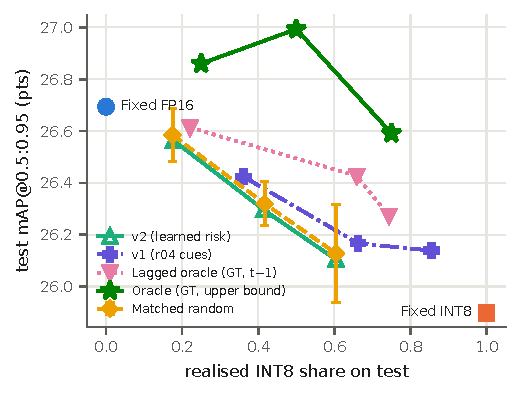
\includegraphics[width=0.62\textwidth]{figs/v2_budgets.pdf}
\caption{Test mAP@0.5:0.95 against the realised INT8 share for the three v2 budgets, with matched random (mean $\pm$ SD over 10 seeds), v1 re-thresholded to each budget, the lagged oracle and the oracle (both use ground truth). Fixed FP16 and INT8 sit at shares 0 and 1. v2 and matched random overlap.}\label{fig:v2budgets}
\end{figure}

% generated by paper/make_tables.py from results/ -- do not edit
\begin{table}[t]
\centering
\caption{Controller v2 follow-up (pre-registered addendum), test split, 40 clips. Budget = target INT8 share set on calib; INT8 frac. = realised test share. Matched random has the realised share and switch rate of v2 at the same budget (mean $\pm$ SD over 10 seeds). Oracle and lagged oracle use ground truth (references, not deployable). 95\% cluster-bootstrap CI over clips. Generated from results/ at commit 2f0c780d.}
\label{tab:v2-budgets}
\scriptsize
\begin{tabular}{lrrrrr}
\toprule
Budget & Policy & mAP50-95 & 95\% CI & INT8 frac. & switches/100 \\
\midrule
-- & Fixed FP16 & 26.69 & [22.96, 36.77] & 0.00 & 0.00 \\
-- & Fixed INT8 & 25.90 & [22.19, 35.93] & 1.00 & 0.00 \\
-- & Fixed FP32 & 26.70 & -- & 0.00 & 0.00 \\
25\% & v2 (learned risk) & 26.56 & [22.90, 36.81] & 0.18 & 2.17 \\
25\% & Matched random & 26.58 $\pm$ 0.10 & [22.85, 36.59] & 0.17 & 2.14 \\
25\% & v1 (r04 cues) & 26.42 & -- & 0.36 & 7.89 \\
25\% & Lagged oracle (GT, t−1) & 26.61 & -- & 0.22 & 30.55 \\
25\% & Oracle (GT, upper bound) & 26.86 & -- & 0.25 & 33.16 \\
50\% & v2 (learned risk) & 26.30 & [22.64, 36.38] & 0.41 & 21.41 \\
50\% & Matched random & 26.32 $\pm$ 0.09 & [22.65, 36.32] & 0.42 & 21.47 \\
50\% & v1 (r04 cues) & 26.17 & [22.46, 35.97] & 0.66 & 7.66 \\
50\% & Lagged oracle (GT, t−1) & 26.43 & -- & 0.66 & 35.77 \\
50\% & Oracle (GT, upper bound) & 26.99 & -- & 0.50 & 35.52 \\
75\% & v2 (learned risk) & 26.10 & [22.48, 36.22] & 0.60 & 3.32 \\
75\% & Matched random & 26.13 $\pm$ 0.19 & [22.42, 36.38] & 0.60 & 3.34 \\
75\% & v1 (r04 cues) & 26.14 & -- & 0.86 & 3.82 \\
75\% & Lagged oracle (GT, t−1) & 26.27 & -- & 0.74 & 32.44 \\
75\% & Oracle (GT, upper bound) & 26.59 & -- & 0.75 & 31.84 \\
\bottomrule
\end{tabular}
\end{table}

% generated by paper/make_tables.py from results/ -- do not edit
\begin{table}[t]
\centering
\caption{Paired cluster-bootstrap differences on the test split, mAP@0.5:0.95 (points), 1000 resamples over clips, seed 2027. P1 is the pre-registered primary test of the addendum.}
\label{tab:v2-pairs}
\scriptsize
\begin{tabular}{lrrr}
\toprule
Comparison & Δ (boot. mean) & 95\% CI & Result \\
\midrule
P1 (primary): v2 − matched random, 50\% & -0.030 & [-0.487, 0.377] & includes 0 \\
P2: v2 − matched random, 25\% & 0.020 & [-0.146, 0.222] & includes 0 \\
P2: v2 − matched random, 75\% & -0.115 & [-1.080, 0.420] & includes 0 \\
P3: v2 − v1, 50\% & 0.177 & [-0.135, 0.557] & includes 0 \\
v2 (50\%) − fixed FP16 & -0.443 & [-1.067, 0.037] & includes 0 \\
v2 (50\%) − fixed INT8 & 0.403 & [-0.129, 0.899] & includes 0 \\
\bottomrule
\end{tabular}
\end{table}


\subsection{Latency and energy under mixed switching}\label{sec:energy}
The v1 energy runs happened to contain only INT8 decisions, so they measured the cost of the adaptive infrastructure rather than switching (Table~\ref{tab:energy}). For v2 we measured \VEnergyClips{} seeded test clips at the 50\% budget, with a realised INT8 share of \VMeasFracINTeight{} and \VMeasSwitchRate{} switches per 100 frames (Fig.~\ref{fig:v2energy}, Table~\ref{tab:v2-energy}). Live decisions matched replay on \VLiveAgreementPct\% of frames.

Forced alternation between INT8 and FP16 on every frame costs \VLatAlternation{} ms and \VETotalAlternation{} mJ per frame, between the two fixed engines. So switching itself is cheap. The controller is not. Computing the cues on a CPU worker hides their \VCueWaitMsSeq{} ms (wait \VCueWaitMsPipe{} ms), but feature statistics and model prediction add \VControllerMsPipe{} ms per frame on the critical path, and the worker competes with the inference thread for the CPU. As a result, adaptive inference took \VLatVTwoPipe{} ms and \VETotalVTwoPipe{} mJ per frame against \VLatFPsixteen{} ms and \VETotalFPsixteen{} mJ for fixed FP16 (P5 \VPFiveResult). The idle-subtracted $E_{\text{dyn}}$ would rank the adaptive configurations as the most efficient, which illustrates why we report $E_{\text{total}}$ as primary.

\begin{figure}[t]
\centering
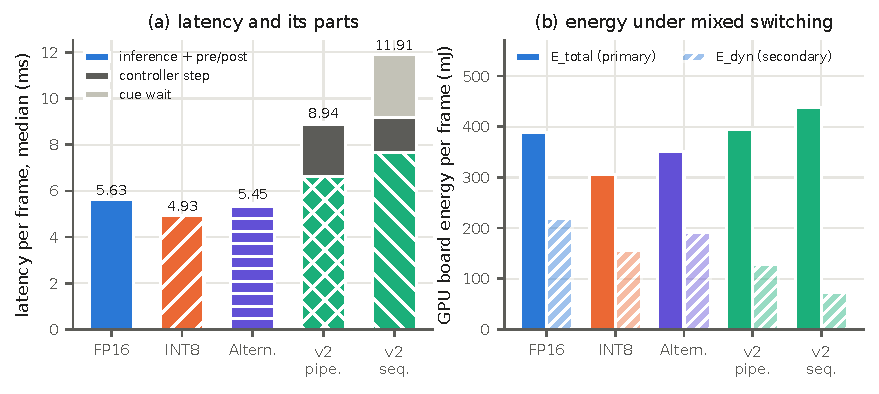
\includegraphics[width=\textwidth]{figs/v2_energy.pdf}
\caption{Live latency per frame split into inference, controller step and cue wait (a), and GPU board energy per frame (b) under mixed switching. $E_{\text{total}}$ is primary; hatched bars show the idle-subtracted $E_{\text{dyn}}$.}\label{fig:v2energy}
\end{figure}

% generated by paper/make_tables.py from results/ -- do not edit
\begin{table}[t]
\centering
\caption{Live measurement under mixed switching on 6 seeded test clips (856 frames, pre-decoded), one Tesla T4, 3 interleaved repeats; median [min--max]. E\_total/frame primary, E\_dyn/frame secondary (NVML board energy counter). Cue wait and controller step (feature statistics + model prediction) are median ms per frame. Live decisions matched replay on 100\% of frames.}
\label{tab:v2-energy}
\scriptsize
\begin{tabular}{lrrrrrrr}
\toprule
Configuration & latency ms & E\_total mJ/frame & E\_dyn mJ/frame & INT8 frac. & switches/100 & cue wait ms & controller ms \\
\midrule
Fixed FP16 & 5.63 [5.63--5.64] & 388.3 [387.8--388.4] & 219.1 [218.7--219.3] & -- & -- & -- & -- \\
Fixed INT8 & 4.93 [4.93--4.93] & 305.2 [303.6--305.2] & 156.6 [155.6--157.3] & -- & -- & -- & -- \\
Forced alternation (every frame) & 5.45 [5.44--5.46] & 350.7 [350.0--350.9] & 192.1 [191.7--192.9] & 0.50 & 100.0 & -- & -- \\
v2 50\%, pipelined cues & 8.94 [8.93--8.98] & 395.0 [392.4--395.2] & 127.5 [127.1--128.5] & 0.37 & 24.3 & 0.05 & 2.29 \\
v2 50\%, sequential cues & 11.91 [11.86--11.98] & 438.5 [434.5--446.8] & 72.5 [70.9--82.7] & 0.38 & 24.2 & 2.73 & 1.53 \\
\bottomrule
\end{tabular}
\end{table}

% generated by paper/make_tables.py from results/ -- do not edit
\begin{table}[t]
\centering
\caption{Measured on one Tesla T4 (live, frames pre-decoded), 3 interleaved repeats of ≥60 s after ≥20 s warm-up; median [min--max] over repeats. Energy from the NVML board energy counter (nvml\_energy\_counter): E\_total/frame is primary; E\_dyn/frame = (ΔE − P\_idle·T)/N is secondary (idle-subtraction favours configurations that leave the GPU waiting, see DEVIATIONS.md V1). GPU board energy only.}
\label{tab:energy}
\scriptsize
\begin{tabular}{lrrrrrrr}
\toprule
Configuration & latency ms (median) & p95 ms & fps & E\_total mJ/frame & E\_dyn mJ/frame & power W & INT8 frac. \\
\midrule
Fixed FP32 & 11.02 [10.95--11.03] & 11.44 & 90.7 & 722.9 [720.9--724.3] & 364.8 [357.7--384.8] & 65.7 & -- \\
Fixed FP16 & 5.78 [5.76--5.79] & 6.07 & 171.8 & 392.5 [392.3--393.9] & 203.8 [199.1--215.2] & 67.6 & -- \\
Fixed INT8 & 5.03 [5.03--5.04] & 5.34 & 197.0 & 332.5 [331.8--332.8] & 166.7 [164.1--177.1] & 65.6 & -- \\
Adaptive, sequential cues & 8.85 [8.83--8.90] & 9.50 & 112.1 & 369.0 [368.8--369.5] & 79.0 [71.4--96.3] & 41.3 & 1.00 \\
Adaptive, pipelined cues & 5.54 [5.52--5.55] & 6.57 & 175.0 & 363.4 [361.2--366.2] & 177.8 [172.7--190.9] & 63.7 & 1.00 \\
\bottomrule
\end{tabular}
\end{table}


%% =====================================================================================
\section{Discussion}\label{sec:discussion}
Three observations explain the negative result. First, the accuracy cost of INT8 on this detector is small and diffuse: about one point of mAP spread over frames, not concentrated in recognisable scenes. Second, the information available before a frame is processed predicts that cost poorly (rank correlation \VSpearman), and even ground truth from the previous frame recovers little of the oracle's headroom. Third, the decision has to cost much less than the \EngineSavingINTeightMs\,ms per frame of engine time that INT8 saves on a T4. A controller that runs Python feature code and a tree model per frame cannot afford that, whereas switching between resident engines costs almost nothing.

A per-frame precision controller would need a much cheaper decision rule (for example, one computed on the GPU or amortised over many frames), a predictor that sees information correlated with INT8 error (for example, the detector's own intermediate activations), or a larger accuracy gap between precisions than YOLO11s shows here. Until then, the practical recommendation for this kind of deployment is fixed INT8, or fixed FP16 where its accuracy is required.

%% =====================================================================================
\section{Limitations and threats to validity}\label{sec:limitations}
\begin{itemize}
\item \textbf{Scope.} One detector (YOLO11s), one dataset (BDD100K MOT, validation-derived clips), one GPU (T4), one quantization recipe (TensorRT post-training INT8 and FP16), GPU board energy only, no embedded device. The results should not be generalised beyond this setting.
\item \textbf{Splits.} Calibration and test clips are disjoint but both come from the official validation split. Day and night strata come from luminance because the tracking labels have no time-of-day attribute.
\item \textbf{Locking at the tolerance boundary.} The v1 lock was \CalibDropMain{} points below FP16 on calibration and \DropAdaptiveVsFPsixteen{} on test. Following the pre-registration, we did not re-tune or re-lock.
\item \textbf{Engine rebuilds.} TensorRT INT8 calibration is not bit-reproducible across builds: the rebuilt INT8 engines differed from the first build by \DriftINTeight{} and \VDriftINTeight{} points of calibration mAP. Each run uses one engine set throughout.
\item \textbf{Post-hoc decisions.} Two decisions were taken after seeing results and are documented as deviations: $E_{\text{total}}$ instead of $E_{\text{dyn}}$ as the primary energy metric, and evaluating H3 on the persistence sweep (a sensitivity analysis). The v2 follow-up was designed after the primary result but pre-registered before it ran.
\item \textbf{References that use ground truth.} The oracle and lagged oracle are not deployable. The size of their headroom depends on the per-frame F1 adequacy rule.
\item \textbf{Synthetic scene changes} and few natural ones. The scene-change benefit of v1 should not be read as evidence for natural cuts.
\end{itemize}

%% =====================================================================================
\section{Conclusion}\label{sec:conclusion}
Under a pre-registered protocol, neither a hand-weighted content-cue controller nor a learned per-frame risk estimator beat cost-matched random placement of INT8 frames for YOLO11s on BDD100K driving video on an NVIDIA T4, although an oracle shows that up to \VHeadroomFiftyPts{} points of mAP are available. Switching precision between resident engines is cheap, but deciding per frame cost more than INT8 saves. Fixed INT8 was the better trade-off in our setting. We release the protocol, locked configurations and result files so that per-frame precision controllers can be tested against the same baselines.

\backmatter

\bmhead{Acknowledgements}
We thank Dr.~Uma Gurav, Head of the Department of Computer Science and Engineering (Artificial Intelligence and Machine Learning), KIT's College of Engineering, Kolhapur, for her guidance as faculty guide. Code and parts of this manuscript were drafted with the assistance of an AI system (Claude, Anthropic). The authors reviewed and verified all code, results and text and take full responsibility for them.

\section*{Declarations}
\begin{itemize}
\item \textbf{Funding:} [to be completed by the authors]
\item \textbf{Competing interests:} The authors declare no competing interests. [authors to confirm]
\item \textbf{Ethics approval and consent to participate:} Not applicable; the study uses a public driving dataset under its research licence.
\item \textbf{Data availability:} BDD100K is available from its authors under the BDD100K licence; we do not redistribute images or labels. Clip identifiers, per-frame statistics and all result files are released with the code.
\item \textbf{Code availability:} The code, locked configurations with SHA-256 hashes, and the scripts that generate every table and figure are released under AGPL-3.0, because the detector framework is AGPL-licensed. [repository URL to be added]
\item \textbf{Author contribution:} [to be completed by the authors]
\end{itemize}

\begin{appendices}
\section{Ablations, persistence sweep and calibration details}\label{app:details}
% generated by paper/make_tables.py from results/ -- do not edit
\begin{table}[t]
\centering
\caption{Ablations on the test split. Each variant was re-calibrated on calib with the same procedure and locked before test ($\delta$ = 0.5 pts); $\delta$ rows are the Pareto locks. Δ vs the locked main controller, in points.}
\label{tab:ablations}
\scriptsize
\begin{tabular}{lrrrrrr}
\toprule
ID & Variant & mAP50-95 & Δ vs main & INT8 frac. & switches/100 & calib \\
\midrule
A-asym & asymmetric persistence (K\_up = 1) & 25.84 & 0.02 & 0.95 & 1.73 & feasible \\
A-c & leave out clutter & 25.81 & 0.00 & 0.96 & 1.48 & feasible \\
A-ema & no EMA (alpha = 1) & 25.81 & 0.00 & 0.96 & 1.48 & feasible \\
A-hyst & no persistence (K = 1) & 25.81 & 0.00 & 0.96 & 1.48 & feasible \\
A-m & leave out motion & 25.89 & 0.07 & 0.90 & 2.24 & feasible \\
A-n & leave out count & 25.86 & 0.05 & 0.58 & 1.94 & feasible \\
A-s & leave out scene-change cue & 25.82 & 0.00 & 0.96 & 1.48 & feasible \\
A-sc-override & scene-change override off & 25.81 & -0.01 & 0.98 & 1.06 & feasible \\
A-u & leave out uncertainty & 25.81 & 0.00 & 0.96 & 1.48 & feasible \\
S-c & clutter only & 25.58 & -0.23 & 0.78 & 1.35 & feasible \\
S-m & motion only & 25.75 & -0.07 & 0.64 & 1.81 & feasible \\
S-n & count only & 25.87 & 0.05 & 0.92 & 1.92 & feasible \\
S-s & scene-change cue only & 26.71 & 0.90 & 0.00 & 0.00 & feasible \\
S-u & uncertainty only & 26.25 & 0.44 & 0.61 & 4.16 & feasible \\
delta0.25 & locked at $\delta$ = 0.25 pts & 25.88 & 0.06 & 0.95 & 1.68 & infeasible \\
delta0.5 & locked at $\delta$ = 0.5 pts & 25.81 & 0.00 & 0.96 & 1.48 & feasible \\
delta1.0 & locked at $\delta$ = 1.0 pts & 25.82 & 0.01 & 0.96 & 1.09 & feasible \\
delta2.0 & locked at $\delta$ = 2.0 pts & 25.82 & 0.01 & 0.96 & 1.09 & feasible \\
\bottomrule
\end{tabular}
\end{table}

% generated by paper/make_tables.py from results/ -- do not edit
\begin{table}[t]
\centering
\caption{Sensitivity analysis (H3): persistence K varied with $\theta$ fixed at the locked value (no re-calibration), test split. The locked controller uses K = 1.}
\label{tab:ksweep}
\scriptsize
\begin{tabular}{lrrrr}
\toprule
K & mAP50-95 & Δ vs K=1 & switches/100 & INT8 frac. \\
\midrule
1 & 25.81 & 0.000 & 1.48 & 0.96 \\
2 & 25.82 & 0.003 & 1.30 & 0.96 \\
3 & 25.81 & -0.004 & 1.21 & 0.95 \\
5 & 25.84 & 0.023 & 1.18 & 0.93 \\
8 & 25.96 & 0.143 & 1.03 & 0.92 \\
\bottomrule
\end{tabular}
\end{table}

% generated by paper/make_tables.py from results/ -- do not edit
\begin{table}[t]
\centering
\caption{Calibration on the calib split only (PLAN §3.5) and the locked main configuration. The lock sat at the $\delta$ limit on calib and did not hold on test (limitation, DEVIATIONS.md L1).}
\label{tab:calibration}
\scriptsize
\begin{tabular}{lr}
\toprule
Item & Value \\
\midrule
configurations searched (Stage A) & 32376 \\
configurations scored with mAP (Stage B) & 20 \\
status (calib) & feasible \\
FP16 calib mAP50-95 & 26.87 \\
locked calib mAP50-95 & 26.44 \\
calib drop vs FP16 (pts; $\delta$ = 0.5) & 0.44 \\
weights (m, c, n, u, s) & 0.25, 0.00, 0.50, 0.00, 0.25 \\
$\theta$ / $\alpha$ / $\theta$\_sc / K\_up / K\_down / H & 0.6118 / 1.0 / 0.5 / 1 / 1 / 3 \\
calib INT8 fraction / switches per 100 & 0.960 / 1.80 \\
engine latency INT8 / FP16 (ms, microbench) & 1.990 / 2.697 \\
switch penalty (ms) & -0.078 \\
sequential cue cost (ms/frame) & 2.696 \\
locked config SHA-256 & 16a1faf1ab9b3c93… \\
\bottomrule
\end{tabular}
\end{table}

% generated by paper/make_tables.py from results/ -- do not edit
\begin{table}[t]
\centering
\caption{Controller v2 fitted and locked on the calib split only (prereg addendum).}
\label{tab:v2-calibration}
\scriptsize
\begin{tabular}{lr}
\toprule
Item & Value \\
\midrule
risk model & gradient-boosted regression trees learning\_rate=0.05, max\_depth=2, max\_iter=100 \\
training rows (calib frames × 2 histories) & 7900 \\
held-out Spearman(pred., true gain), clip-grouped CV & 0.060 \\
FP16 calib mAP50-95 & 26.88 \\
budget 25\%: K / calib INT8 frac. / calib mAP50-95 & 3 / 0.250 / 26.65 \\
budget 50\%: K / calib INT8 frac. / calib mAP50-95 & 1 / 0.500 / 25.97 \\
budget 75\%: K / calib INT8 frac. / calib mAP50-95 & 3 / 0.750 / 25.98 \\
rebuilt-engine drift vs Step 2 (calib mAP50-95, pts) & fp32 0.00, fp16 0.06, int8 0.41 \\
\bottomrule
\end{tabular}
\end{table}

% generated by paper/make_tables.py from results/ -- do not edit
\begin{table}[t]
\centering
\caption{Paired differences on the test split (points): full-data point estimate, bootstrap mean and 95\% cluster-bootstrap CI over the 40 clips (1000 resamples, seed 2027); random groups use the per-resample mean over 10 seeds. Adaptive − K=1 is identically 0 because the locked controller has K = 1.}
\label{tab:ci-pairs}
\scriptsize
\begin{tabular}{lrrrrrr}
\toprule
Difference & Δ mAP50-95 & boot. mean & 95\% CI & excludes 0 & Δ mAP50 & 95\% CI \\
\midrule
Adaptive (locked) − Adaptive K=1 & 0.000 & 0.000 & [0.000, 0.000] & no & 0.000 & [0.000, 0.000] \\
Adaptive (locked) − Fixed FP16 & -0.895 & -0.998 & [-2.420, -0.127] & yes & -1.711 & [-3.046, -0.395] \\
Adaptive (locked) − Fixed INT8 & 0.050 & 0.030 & [-0.531, 0.267] & no & -0.038 & [-0.683, 0.299] \\
Adaptive (locked) − i.i.d. random (10 seeds) & -0.343 & -0.378 & [-1.375, 0.212] & no & -0.801 & [-1.832, 0.126] \\
Adaptive (locked) − Matched random (10 seeds) & 0.044 & 0.007 & [-0.702, 0.270] & no & -0.024 & [-0.894, 0.336] \\
Oracle-cheap (uses GT) − Fixed FP16 & -0.034 & -0.097 & [-0.549, 0.482] & no & 0.334 & [-0.884, 0.937] \\
\bottomrule
\end{tabular}
\end{table}

% generated by paper/make_tables.py from results/ -- do not edit
\begin{table}[t]
\centering
\caption{Provenance and measurement details (all values from results/).}
\label{tab:provenance}
\scriptsize
\begin{tabular}{lr}
\toprule
Item & Value \\
\midrule
BDD subsets (Step 1) & 098a7257 \\
Step 2 eval / 02b diagnostic & 18f62138 / 4d37cc15 \\
Notebook 04 run (clean checkout) & 4e35b3e1 (dirty=False) \\
GPU / driver / CUDA & Tesla T4 / 580.178.04 / 13.0 \\
torch / ultralytics / tensorrt & 2.11.0+cu130 / 8.4.216 / 10.16.1.11 \\
rebuilt-engine drift vs Step 2, calib mAP50-95 (max over slices, pts) & fp32 0.000, fp16 0.083, int8 0.213 \\
engine SHA-256 (FP32 / FP16 / INT8) & 7d32b8d1ce78 / 2ad8fc60a77a / 2cc6f201db4a \\
GPU memory, engine alone (MiB) FP32 / FP16 / INT8 & 124 / 76 / 66 \\
GPU memory, adaptive set INT8+FP16 (MiB) & 140 \\
live vs replay (test subset): level agreement / |Δ mAP50-95| pts & 1.000 / 0.000 (1924 frames) \\
\bottomrule
\end{tabular}
\end{table}

\end{appendices}

\bibliography{refs}

\end{document}
